\documentclass[11pt]{article}

\usepackage[a4paper,margin=29mm]{geometry}
\usepackage[T1]{fontenc}
\usepackage{lmodern}
\usepackage{microtype}
\usepackage{amsmath,amssymb,amsthm,mathtools}
\usepackage{array,booktabs}
\usepackage{enumitem}
\usepackage{float}
\usepackage{needspace}
\usepackage{tikz}
\usetikzlibrary{arrows.meta,positioning}
\usepackage[hidelinks]{hyperref}


\newtheorem{theorem}{Theorem}[section]
\newtheorem{proposition}[theorem]{Proposition}
\newtheorem{lemma}[theorem]{Lemma}
\theoremstyle{definition}
\newtheorem{definition}[theorem]{Definition}
\theoremstyle{remark}
\newtheorem{remark}[theorem]{Remark}

\newcommand{\F}{\mathbb F}
\newcommand{\PG}{\operatorname{PG}}
\newcommand{\PGL}{\operatorname{PGL}}
\newcommand{\Aut}{\operatorname{Aut}}
\newcommand{\cC}{\mathcal C}
\newcommand{\supp}{\operatorname{supp}}

\title{Reconstructing $\PG(2,13)$, its conic, and polarity\\
from the minimum words of a binary conic code}
\author{Tavis Rudd}
\date{August 2026}

\begin{document}
\begingroup
\makeatletter
\let\clebschmaintitle\@title
\def\@title{\par\vspace*{12mm}\noindent
  \LARGE\clebschmaintitle}
\makeatother
\maketitle
\endgroup

\begin{abstract}
How little of an incidence code is needed to reconstruct the geometry that
produced it?  Let \(K\) be the binary nullspace of the
passant-by-internal incidence matrix of a nonsingular conic in
\(\PG(2,13)\).  We prove that \(K\) has parameters \([78,36,12]_2\) and
exactly \(364\) minimum words.  They form four
\(\PGL(2,13)\)-orbits---one octahedral family and three chord-indexed
punctured-conic families---and every orbit spans \(K\).

Weighted pair concurrences in these minimum supports recover the \(78\)
passant incidence rows, the code, and the six-class elliptic association
scheme.  Pair parity recovers \(K\), while unary minimum-support statistics
are constant; reconstruction therefore has exact arity two.  The recovered
scheme has automorphism group \(\PGL(2,13)\).  Its Sylow-\(13\) subgroups and
involutions then reconstruct all \(183\) points and lines of
\(\PG(2,13)\), the distinguished conic, and its polarity, without coordinates
or a projective frame.  The binary relation algebra acts on \(K\) through
\(\F_8\), making it twelve-dimensional over that field.

The distance proof reduces weight eight to a positive-semidefinite clique
obstruction and weight ten to two line-moment profiles followed by bounded
stabilizer exhaustion.  The theorem is intentionally specific to \(q=13\):
it gives complete ambient reconstruction, not a uniform distance formula.
\end{abstract}

\noindent\textbf{Keywords.} binary conic code; passant line; minimum-weight
codeword; weighted hypergraph \(2\)-section; projective-plane reconstruction;
elliptic association scheme; polarity; automorphism group.

\smallskip
\noindent\textbf{2020 Mathematics Subject Classification.} 94B05, 51E20,
05B25, 05E30.

\section{Introduction and statement}

We ask how little of an incidence code is needed to reconstruct the geometry
that produced it.  This is a fixed-field inverse problem: starting from the
minimum-support hypergraph, we ask for the least arity of support data needed
to reconstruct the geometry erased by row reduction.  The retained input is
only the weighted pair data inside the minimum supports of a binary code;
neither its parity-check matrix nor an ambient projective plane is supplied.
At \(q=13\) this pairwise shadow is complete: it recovers the incidence
matrix, the elliptic association scheme, the full automorphism group, and
finally the marked conic plane and its polarity.  Unary data are constant
there, while weighted pair data recover that plane and its polarity, so the
exact arity is two.

Fix a nonsingular conic \(\cC\subset\PG(2,13)\).  A line is
\emph{passant} when it is disjoint from \(\cC(\F_{13})\).  Conic polarity
identifies the \(78\) internal points with the \(78\) passant lines.  Let
\(M\) be their binary incidence matrix and put
\[
 K=\ker_{\F_2}M\subseteq\F_2^{78}.
\]
Write \(G_0=\PGL(2,13)\) for the conic stabilizer in its natural action.
The coordinate set is the set of internal points.  Automorphisms below are
coordinate permutations preserving the indicated code or minimum-support
system.

Let
\[
 \mathcal H=\{\supp(c):c\in K,\ \operatorname{wt}(c)=12\}
\]
be the minimum-support hypergraph on the unlabeled coordinate set of \(K\).

\begin{theorem}[Minimum words recover the conic plane]
\label{thm:main}
The code \(K\) has parameters \([78,36,12]_2\) and exactly \(364\)
minimum words.  Under \(\PGL(2,13)\), those words form four orbits of
size \(91\).  One is an octahedral homogeneous space with stabilizer
\(S_4\); the other three are chord-indexed punctured conics with stabilizer
\(D_{24}\).  Every orbit spans \(K\).

Let \(c(P,Q)\) be the number of minimum supports containing \(P,Q\).
The neighborhoods defined by \(c(P,Q)=8\) are exactly the \(78\) rows of
\(M\).  The other five elliptic relations are recovered from the remaining
pair weights and one common-neighbor count.  Moreover, if
\((R_{\mathcal H})_{PQ}=c(P,Q)\bmod2\) off the diagonal and
\((R_{\mathcal H})_{PP}=0\), then
\(\operatorname{im}R_{\mathcal H}=K\).  Thus the weighted \(2\)-section of
\(\mathcal H\) reconstructs the incidence matrix, code, and elliptic scheme.

From the reconstructed group, its fourteen Sylow-\(13\) subgroups and
\(169\) involutions recover all \(183\) points and lines of
\(\PG(2,13)\), the distinguished conic, and its polarity.  Consequently
weighted-pair reconstruction has exact arity two, and
\[
 \Aut(K)=\Aut(\mathcal H)=\PGL(2,13)
\]
in its symmetric-square action on the \(78\) internal points.
\end{theorem}

Reconstruction is intrinsic, not coordinatized.  It recovers the marked
plane and polarity up to isomorphism, but it does not choose an ordered
projective frame, a field labeling, or an equation for the conic.  Such a
choice is necessarily noncanonical: the \(2184\) ordered triples of distinct
conic points form a torsor for \(\PGL(2,13)\).

\medskip
\noindent\textbf{Proof and reading map.}
\begin{center}
\footnotesize
\setlength{\tabcolsep}{3pt}
\renewcommand{\arraystretch}{0.9}
\begin{tabular}{@{}c c c@{}}
\fbox{\parbox{0.27\textwidth}{\centering
Weight eight gives a seven-clique in the tangent graph; the rank-28
positive semidefinite form bounds its cliques by five.\\[-1pt]
\emph{Section~\ref{sec:distance}}}}
&&
\fbox{\parbox{0.27\textwidth}{\centering
The line moment reduces weight ten to two shapes; stabilizer calculations
exclude both.\\[-1pt]
\emph{Section~\ref{sec:distance}}}}
\\
\(\searrow\) && \(\swarrow\)\\
&
\fbox{\parbox{0.35\textwidth}{\centering
Distance is twelve.  Fixed-point exhaustion and projective transport give
364 minimum supports in four geometric orbits.\\[-1pt]
\emph{Section~\ref{sec:minimum-geometry}}}}
&\\
& \(\Downarrow\) &\\
&
\fbox{\parbox{0.35\textwidth}{\centering
Weighted pairs in the minimum supports recover the six elliptic relations.\\[-1pt]
\emph{Section~\ref{sec:minimum-geometry}}}}
&\\
\(\swarrow\) && \(\searrow\)\\
\fbox{\parbox{0.27\textwidth}{\centering
Concurrence-eight neighborhoods recover the incidence rows; pair parity
recovers the code.\\[-1pt]
\emph{Section~\ref{sec:minimum-geometry}}}}
&&
\fbox{\parbox{0.27\textwidth}{\centering
Relation operators recover the \(\F_8\)-action, orbit spanning, and
\(\PGL(2,13)\).\\[-1pt]
\emph{Section~\ref{sec:hidden-field}}}}
\\
\(\searrow\) && \(\swarrow\)\\
&
\fbox{\parbox{0.35\textwidth}{\centering
Sylow-13 subgroups and involutions recover the ambient plane, conic, and
polarity.\\[-1pt]
\emph{Section~\ref{sec:ambient-plane}}}}
&
\end{tabular}
\end{center}

The reductions are structural except at small exact endpoints.  The finite
leaves are the four line-stabilizer and thirty-three point-stabilizer orbits
in weight ten, the one-point minimum-layer exhaustion, and one bounded
matching-profile check for the octahedral construction.  The recovered
group/plane dictionary is independently replayed in the complete finite
model.

The code belongs to the fixed-conic LDPC family introduced by
Droms--Mellinger--Meyer~\cite{DromsMellingerMeyer2006}.  Their general bounds
specialize here to \(8\le d\le12\)~\cite[Theorem~4.9]{DromsMellingerMeyer2006},
and they report the \(q=13\) parameter \([78,36,12]_2\) in their Table~8.
The later comparison table of Ma--Liu--Tian records the same general
interval~\cite[Table~1]{MaLiuTian2024}.
Madison and Wu proved the general nullity formula
\((q-1)^2/4\)~\cite[Corollary~5.4]{MadisonWu2012}; their module theorem
\cite[Theorem~5.1(i)]{MadisonWu2012} splits
the code over \(\overline{\F_2}\) into three non-isomorphic simple
twelve-dimensional \(\operatorname{PSL}(2,13)\)-modules.  In
Section~\ref{sec:hidden-field} we mark them by the eigenvalues
\(\alpha,\alpha^2,\alpha^4\) of \(A_9\).  Frobenius cycles the three
constituents, so their binary descent is irreducible; Schur descent then gives
endomorphism field \(\F_8\).  The unmarked irreducibility already forces any
nonzero minimum-word orbit to span.  We mark \(A_9\) among the three
conjugates, recover it from pair data, and give direct Gram certificates for
each of the four orbits.

Hollmann and Xiang constructed the elliptic association scheme afforded by
the same conic action~\cite[Sections~3--5]{HollmannXiang2006}, attributing its first
description to Hollmann's thesis~\cite{HollmannThesis1982}.  The identification
of involutions with off-conic points, with involution axis equal to polar line,
is classical and is stated explicitly by Tranchida
\cite[Section~2]{Tranchida2024}.  We prove the reported distance at
\(q=13\), classify all minimum words, and prove that their weighted pair data
recovers these established ambient structures.

\section{Distance twelve}
\label{sec:distance}

We use the model \(\cC:XZ-Y^2=0\).  Every row and column of \(M\) has
weight seven, and conic polarity identifies the two index sets.  The
Madison--Wu formula gives \(\dim K=36\); direct binary elimination is an
independent check of rank \(42\).

Summing all row equations gives the all-one functional, so every word of
\(K\) has even weight.  If a nonzero word contains an internal point \(P\),
each of the seven passants through \(P\) contains a second support point.
Those seven points are distinct.  Thus every nonzero word has weight at
least eight.

\subsection{The tangent obstruction in weight eight}

The mechanism has two steps.  A saturated passant pencil turns a hypothetical
weight-eight support into a seven-clique in a local graph; a
positive-semidefinite form bounds every clique in that graph by five.  On a
first reading, the matrix entries below may be skipped once these two conclusions
and the exact rank certificate are retained.

Suppose that a word has weight eight and fix a support point \(P\).  Each of
the seven passants through \(P\) must contain another support point.  Since
only seven points remain, each passant contains exactly one of them.  Applying
the same argument at every support point shows that every support join is
passant and that no three support points are collinear.  Thus the support is
an eight-arc, and every passant pencil at a support point is saturated.  The
seven remaining lines through each support point are therefore both the
combinatorial tangents to the arc and the conic secants through that point.

For each secant line choose a nonzero linear equation.  For an internal point
\(P\), put
\[
 T_P(X)=\prod_{\substack{\ell\ni P\\
                    \ell\text{ secant to }\cC}}\ell(X).
\]
For a pairwise-passant triple define
\[
 h(P,Q,R)=
 \frac{T_P(Q)T_Q(R)T_R(P)}
      {T_P(R)T_R(Q)T_Q(P)}.
\]
Every displayed evaluation is nonzero because the three joins are passant.
Rescaling a line equation multiplies one numerator and one denominator factor
by the same scalar, so \(h\) is well defined.  The saturated-pencil
identification above makes the factors of \(T_P\) precisely the combinatorial
tangents at \(P\).
Segre's lemma of tangents in the coordinate-free form of
Ball--Lavrauw~\cite[Lemma~27]{BallLavrauw2019} gives
\(h(P,Q,R)=1\) for every triple in the hypothetical support.  Its hypotheses
apply with \(t=13+3-1-8=7\); hence the sign
\((-1)^{t+1}\) is \(+1\).  With
the cyclic order \(P,Q,R\) its tangent-product quotient is exactly the
displayed \(h\) (not its negative; reversing the cycle only inverts it).  Fix
\(P=(1:0:2)\).  Its other seven points would form a clique in the graph on
the \(42\) passant-join neighbors of \(P\), where \(Q\) and \(R\) are
adjacent when \(QR\) is passant and \(h(P,Q,R)=1\).

The projective map
\[
 \gamma(x:y:z)=
 (x+6y+9z:7x+9y+3z:10x+y+z)
\]
fixes \(P\) and has order \(14\) on its passant-join neighbors.  With indices
in \(\mathbf Z/14\), put
\[
 A_i=\gamma^i(1:1:7),\qquad
 B_i=\gamma^i(1:1:6),\qquad
 C_i=\gamma^i(1:2:10).
\]
These three orbits are disjoint and contain all \(42\) neighbors.  Direct
substitution in the product above gives
\[
\begin{array}{c|c}
\text{orbit pair}&j-i\pmod {14}\\ \hline
AA&4,6,8,10\\
AB&6,7,11,12\\
AC&1,3\\
BB&6,8\\
BC&3,5,6,8,9,11\\
CC&2,4,10,12.
\end{array}
\]
Let \(C\) be the symmetric \(42\)-square matrix in the displayed vertex
order, written in \(14\)-square circulant blocks.  Its six upper-block first
rows are
\[
\begin{array}{c|rrrrrrrrrrrrrr}
00&40&9&8&-8&-10&0&-10&-2&-10&0&-10&-8&8&9\\
01&7&6&6&6&7&-1&-10&-10&-8&0&-8&-10&-10&-1\\
02&0&-10&2&-10&0&3&2&9&2&4&2&9&2&3\\
11&40&15&10&10&-6&-3&-10&-22&-10&-3&-6&10&10&15\\
12&-13&3&0&-10&8&-10&-10&14&-10&-10&8&-10&0&3\\
22&40&-9&-10&19&-10&2&8&-12&8&2&-10&19&-10&-9.
\end{array}
\]
The lower blocks are the transposes.  Comparison with the six difference
sets shows that \(C\) has diagonal \(40\) and entry \(-10\) on every edge
of the local graph.

The matrix is positive semidefinite.  Exact cyclic Fourier traces and Newton
identities give
\[
 \chi_C(x)=x^{14}(x^2-94x+279)(x^2-26x+135)f(x)^2g(x)^2,
\]
where
\[
\begin{aligned}
f(x)={}&x^6-247x^5+22466x^4-910807x^3
 +15948097x^2-111043270x+189747571,\\
g(x)={}&x^6-533x^5+105578x^4-9736765x^3
 +438572569x^2-9062718662x+68467048091.
\end{aligned}
\]
Every nonzero factor has alternating coefficients.  Its value at \(-t\) is
therefore positive for \(t\ge0\).  Since \(C\) is real symmetric, it has no
negative eigenvalue; the displayed factorization also gives rank \(28\).
An independent rational Schur elimination gives the same twenty-eight
positive pivots.

If \(v\) is the characteristic vector of a clique of size \(c>0\), then
\[
 0\le v^{\mathsf T}Cv
   =40c-20\binom c2=10c(5-c).
\]
Thus \(c\le5\).  The set
\(\{A_0,B_6,B_{12},C_1,C_3\}\) is a five-clique, so the bound is sharp.
The exact certificate also classifies the extremal five-cliques.  This
sharpening is not used to exclude weight eight.
Its fourteen translates are linearly independent kernel vectors;
nullity fourteen makes them a basis of \(\ker C\).  Equality in the
quadratic-form bound puts every maximum-clique vector in this kernel, and
solving the resulting \(0\)--\(1\) constraints in that basis gives precisely
the fourteen translates.  In particular the seven-clique required by a
weight-eight word cannot occur.

\subsection{The two weight-ten profiles}

Here the conceptual step is the line moment, which reduces every possible
support to two geometric shapes.  The stabilizer calculations that follow
close those two finite leaves and introduce no further shape.

Let \(S\) be a hypothetical weight-ten support, and let \(n_i\) be the
number of passants meeting \(S\) in exactly \(i\) points.  Code parity makes
every occurring \(i\) even, and incidence counting gives
\[
 \sum_i i n_i=70.
\]
At a selected point, pencil parity gives secant degree zero or two.  The
secant graph induced on \(S\) is therefore a union of cycles and isolated
vertices.  If \(m\) is the number of its cycle vertices, then it has \(m\)
edges, and the other \(45-m\) pairs have passant join.  Hence
\[
 \sum_i\binom{i}{2}n_i=45-m.
\]
Subtracting half the first identity yields the decisive moment
\begin{equation}
 4n_4+12n_6+24n_8+\cdots=10-m.       \label{eq:weight-ten-moment}
\end{equation}
No \(n_i\) with \(i\ge6\) can occur.  The degree condition and
\eqref{eq:weight-ten-moment} leave exactly
\[
\begin{array}{c|c|c}
m&(n_2,n_4)&\text{shape}\\ \hline
6&(33,1)&\text{four isolated vertices on one four-point passant and six cycle vertices},\\
10&(35,0)&\text{ten cycle vertices; every passant meets }S\text{ in }0\text{ or }2.
\end{array}
\]
Two degree-two vertices cannot by themselves form a cycle; in the
first case uniqueness of the four-point passant puts all isolated vertices
on that line.

The first shape has only four normalized cases.  The effective stabilizer of
a passant acts as \(D_{14}\) on its seven internal points, with four orbits
on four-subsets:
\[
\begin{array}{c|c|c|c}
\text{representative}&\text{orbit size}&|X|&
 \text{secant degrees in }X\\ \hline
0123&7&7&(3,3,4,4,4,4,4)\\
0124&14&3&(0,0,0)\\
0134&7&5&(2,2,2,4,4)\\
0135&7&5&(2,2,2,3,3).
\end{array}
\]
Here \(X\) is the set of internal points passantly joined to all four fixed
points; retaining the three unused points of the fixed line only enlarges
it.  These four stabilizer orbits exhaust the four-subsets, and none of their
induced secant graphs contains the required six-vertex two-regular subgraph.
Thus the \(m=6\) shape is impossible.

For \(m=10\), fix \(P\in S\).  The remaining points consist of one point in
each of the seven six-point passant fibres through \(P\) and an unordered
pair among its \(35\) secant neighbors.  The stabilizer
\((G_0)_P\cong D_{28}\) has thirty-three orbits on the \(595\) pairs: five of
size \(7\), sixteen of size \(14\), and twelve of size \(28\).  For one
representative of each orbit, add the seven fibre points in order, rejecting
a prefix once a passant contains three selected points or a selected point
has more than two secant neighbors.  The complete certificate has last
surviving-depth mass
\[
\begin{array}{c|rrrrr}
\text{depth}&0&1&2&3&4\\ \hline
\text{pair mass}&28&35&91&238&203.
\end{array}
\]
The masses sum to \(595\), and no representative survives the fifth fibre.
Thus \(m=10\) is impossible as well.

Finally, the twelve internal points
\[
\begin{gathered}
(1:0:2),(1:3:2),(1:4:5),(1:1:8),
(1:4:8),(1:1:7),\\
(1:7:12),(1:3:3),(1:9:11),(1:10:11),
(1:0:5),(1:8:7)
\end{gathered}
\]
have zero syndrome.  Their stabilizer is dihedral of order \(24\).
Therefore \(d(K)=12\).

\section{Minimum geometry and weighted pairs}
\label{sec:minimum-geometry}

Fixed-point exhaustion first proves that there are \(364\) minimum supports in
four orbits; the domain-size ledger may be skipped on a first reading.  The
matching model then identifies the four families, and their pair concurrences recover the
incidence rows and the full elliptic scheme.

Fix one support point \(P\).  Its seven passant fibres again have six eligible
points each, and it has \(35\) secant neighbors.  Pencil parity leaves
\(s=0,2,4\) secant neighbors.
The corresponding multiplicities in the seven passant fibres, followed by
the number of secant neighbors, are
\[
 (5,1^6;0),\qquad (3,3,1^5;0),\qquad
 (3,1^6;2),\qquad (1^7;4).
\]
A syndrome-indexed exact check exhausts these four fixed-point domains.  Its
input sizes are respectively
\[
 7\binom65 6^6,\quad
 \binom72\binom63^2 6^5,\quad
 7\binom63 6^6\binom{35}{2},\quad
 6^7\binom{35}{2}^2,
\]
with disjoint secant pairs in the last domain.  The certificate specifies the
four partitions, proves their coverage, tests zero syndrome, and deduplicates
only after conversion to unordered supports.  The four domains contribute
\(0,0,0,56\) words.  The canonical replay generates the four projective
\(\PGL(2,13)\)-orbits, and intersects each orbit with the supports containing
\(P\).  These four fixed-point slices are disjoint, each has size \(14\), and
their union is checked for equality with the exhaustive \(56\)-word set.
The order-\(28\) stabilizer of the fixed point acts transitively on each
slice; the stabilizer of a support inside it has order \(2\).
Transitivity, or equivalently the count \(56\cdot78/12=364\), proves global
exhaustion.

The replay generates each orbit from its recorded representative and checks
every support against \(M\).  The geometric constructions in
Section~\ref{sec:minimum-families} identify those orbits without
representatives.

\subsection{One octahedral and three toric families}
\label{sec:minimum-families}

Parametrize the conic by \((t^2:t:1)\), with its usual point at infinity.
An internal point \(P=(x:y:z)\) defines the fixed-point-free involution
\[
 j_P(t)=\frac{yt-x}{zt-y},\qquad
 J_P=\begin{pmatrix}y&-x\\z&-y\end{pmatrix},\qquad
 J_P^2=(y^2-xz)I.
\]
The seven secants through \(P\) are the seven pairs
\(\{t,j_P(t)\}\).  Thus internal points may be read as perfect matchings of
the fourteen conic points.

Fix a chord \(e\), carry its endpoints to \(\{0,\infty\}\), and let
\(N_e\cong D_{24}\) be their setwise stabilizer.  The three supports over
\(e\) are
\[
 S_r(e)=\{(x:1:r^{-1}x^{-1}):x\in\F_{13}^{\times}\},
 \qquad r\in\{2,5,11\}.
\]
The second-conic upper-bound construction is due to
Droms--Mellinger--Meyer~\cite[proof of Theorem~4.9]{DromsMellingerMeyer2006};
here its \(q=13\) instances are separated and classified over each chord.
Intrinsically, these three parameters satisfy
\(\chi(r)=-1\) and \(\chi(r-1)=1\).  The support \(S_r(e)\) is the
punctured pencil conic
\[
 \{y^2=rxz\}(\F_{13})\setminus e,
\]
so it has size twelve and stabilizer exactly \(N_e\).  At each displayed
point, \(\Delta=1-r^{-1}=(r-1)/r\) is a nonsquare; hence all twelve points
are internal.  The set is a codeword for a structural reason.  If a passant
\(AX+BY+CZ=0\) met \(S_r(e)\) with odd multiplicity, the polynomial
\(Ax^2+Bx+C/r\) would have a double root.  Then
\[
 B^2-4AC=B^2(1-r)
\]
would be a square, contrary to the line being passant.  Hence every passant
meets \(S_r(e)\) in zero or two points.  There is no missing endpoint case:
a passant contains neither endpoint of the chord \(e=\{0,\infty\}\), so
\(A,C\ne0\).  Thus neither zero nor infinity is a root, and the displayed
quadratic accounts for the entire intersection with the punctured conic.

For the remaining family, let \(O\le G_0\) be generated by
\(\left(\begin{smallmatrix}1&0\\3&8\end{smallmatrix}\right)\) and
\(\left(\begin{smallmatrix}1&4\\3&0\end{smallmatrix}\right)\).
Exact multiplication gives orders \((4,3,2)\) for the generators and their
product, and \(|O|=24\), so \(O\cong S_4\), with conic orbits of sizes six
and eight.  On all 78 internal points, matching profile \((2,3)\) inside
those orbits selects a unique 12-point suborbit \(X_O\) (and two crossing
pairs).  The leaf checks all 78 passant parities and
\(\operatorname{Stab}_{G_0}(X_O)=O\), identifying the remaining minimum orbit.

All four stabilizers have order \(24\).  Each family therefore has
\(2184/24=91=\binom{14}{2}\) supports, agreeing with the fixed-point
exhaustion above.

\subsection{Exact arity-two reconstruction}
\label{sec:pair-reconstruction}

We now forget how the supports were constructed and retain only their weighted
pair graph.  From that graph alone we recover first the six elliptic relations,
then the incidence rows, and finally the code.

For internal points \(P=(x_P:y_P:z_P)\) and \(Q\), set
\[
 \Delta(P)=y_P^2-x_Pz_P,\qquad
 \beta(P,Q)=2y_Py_Q-x_Pz_Q-z_Px_Q,
\]
and
\[
 \rho(P,Q)=\frac{\beta(P,Q)^2}{\Delta(P)\Delta(Q)}.
\]
On distinct internal points, \(\rho\) takes the six values
\(0,1,3,9,10,12\).  Write \(A_r\) for the adjacency matrix of the
non-diagonal relation \(\rho(P,Q)=r\).

For distinct coordinates put
\[
 c(P,Q)=\#\{S\in\mathcal H:\{P,Q\}\subseteq S\}.
\]
It suffices to count at one point.  Fix
\(P=(1:0:2)\); one representative in each relation is displayed below.
\[
\begin{array}{c|cccccc}
\rho&0&1&3&9&10&12\\ \hline
Q&(1:0:11)&(1:0:5)&(1:0:7)&(1:1:6)&(1:1:7)&(1:2:10)\\
\text{valency}&7&14&14&14&14&14\\
c(P,Q)&8&6&6&12&7&9.
\end{array}
\]
Direct counting of the four intrinsic support representatives gives these
entries; transitivity on every relation transports them to all pairs.  The
four generated support orbits have size \(91\), are disjoint, and deduplicate
to all \(364\) minimum supports.  As a global check, the numbers of unordered
pairs with concurrence \(8,6,12,7,9\) are respectively
\(273,1092,546,546,546\).  The exact replay is
\nolinkurl{verification/verify_pair_reconstruction.py}, with compact output
in \nolinkurl{verification/pair_reconstruction.json}.
Only the relations \(A_1\) and \(A_3\) are fused.  For a concurrence-six
pair define
\[
 d_7(P,Q)=\#\{R:c(P,R)=c(R,Q)=7\}.
\]
The \(A_{10}^2\) intersection row gives
\[
 d_7(P,Q)=2\quad\text{on }A_1,
 \qquad d_7(P,Q)=4\quad\text{on }A_3.
\]
This pair-derived common-neighbor count recovers the full six-relation elliptic
scheme.

\smallskip
\noindent\emph{Comparison with Hollmann--Xiang.}
Let \(u\) be their cross ratio, modulo inversion, and let
\(\lambda=f(u)=1/4+1/(-2+u+u^{-1})\) be their modified label.  After swapping
their first two conic coordinates and passing from points to polar lines,
their cross-ratio formula~\cite[Theorem~5.3]{HollmannXiang2006} gives
\[
 \lambda=\widehat\rho_{\rm HX}(P^\perp,Q^\perp)=9\rho(P,Q).
\]
Thus the source-to-paper dictionary is
\[
\begin{array}{c|rrrrrr}
\{u,u^{-1}\}&\{12,12\}&\{4,10\}&\{3,9\}&\{5,8\}&\{2,7\}&\{6,11\}\\ \hline
\lambda&0&9&1&3&12&4\\
\text{paper relation}&A_0&A_1&A_3&A_9&A_{10}&A_{12}.
\end{array}
\]

The concurrence-eight relation recovers the incidence rows directly.
Polarity sends
\(P=(x:y:z)\) to \(P^\perp=(-z:2y:-x)\), and
\[
 Q\in P^\perp
 \iff \beta(P,Q)=0
 \iff \rho(P,Q)=0
 \iff c(P,Q)=8.
\]
Consequently the seventy-eight concurrence-eight neighborhoods are exactly
the seventy-eight rows of \(M\).

The pair data also recovers the code without first naming a row.  Let
\((R_{\mathcal H})_{PQ}=c(P,Q)\bmod2\) off the diagonal and
\((R_{\mathcal H})_{PP}=0\).  Then
\[
 R_{\mathcal H}=A_{10}+A_{12},\qquad
 \operatorname{rank}R_{\mathcal H}=36,
 \qquad A_0R_{\mathcal H}=0,
\]
so \(\operatorname{im}R_{\mathcal H}=K\).  Every coordinate occurs in
\(364\cdot12/78=56\) minimum supports, making unary data constant.  Pair
data suffices and unary data does not; reconstruction arity is exactly two.
Indeed, intrinsic reconstruction is equivariant: the constant unary datum
has automorphism group \(S_{78}\), whereas Section~\ref{sec:hidden-field}
proves that the recovered marked presentation has automorphism group
\(\PGL(2,13)\).  No intrinsic reconstruction of those nontrivial marked
relations can therefore factor through unary data.
Here ``recovers'' means the marked code--hypergraph presentation up to
isomorphism.  It does not choose an ordered projective frame or a labeling of
the ground field.

\section{The hidden field, spanning, and automorphisms}
\label{sec:hidden-field}

The recovered pair coloring now becomes an operator algebra.  Its binary
action projects onto \(K\), the single operator \(A_9\) supplies the scalar
field \(\F_8\), and the four orbit Grams become invertible scalars.  The final
anchor argument determines the full permutation group.  For a first reading,
the integral table may be skipped after retaining its binary action on \(K\)
and the cubic satisfied by \(A_9\).

These six level relations form the elliptic scheme.  Polarity identifies
\(A_0\) with \(M\), up to row order.

Only the following integral intersection rows are used:
\[
\begin{array}{c|rrrrrrr}
 &I&A_0&A_1&A_3&A_9&A_{10}&A_{12}\\ \hline
A_0^2   &7&0&0&0&1&1&1\\
A_0A_9  &0&2&2&2&0&2&0\\
A_0A_{10}&0&2&2&0&2&0&2\\
A_0A_{12}&0&2&0&2&0&2&2\\
A_9^2   &14&0&4&2&2&1&4\\
A_{10}^2&14&0&2&4&2&4&1\\
A_{12}^2&14&4&2&2&3&2&2.
\end{array}
\]
These numbers come from fixing \(P=(1:0:2)\), using the six relation
representatives in Section~\ref{sec:pair-reconstruction}, and counting
intermediate internal points.
Transitivity on each ordered relation makes those seven representative rows
the full matrix identities.  Reducing modulo two gives
\begin{equation}
\label{eq:scheme}
\begin{split}
 A_0^2&=I+A_9+A_{10}+A_{12},\\
 A_0A_r&=0\quad(r=9,10,12),\\
 A_1(A_9+A_{10}+A_{12})&=0,\qquad
 A_3(A_9+A_{10}+A_{12})=0,\\
 A_9^2&=A_{10},\qquad A_{10}^2=A_{12},\qquad A_{12}^2=A_9.
\end{split}
\end{equation}
These are parity reductions of intersection numbers.  The
\(\PGL(2,13)\)-action is transitive on each relation, so fixing one point and
substituting one representative of every relation checks all entries.

Put \(B=A_9\) and
\[
 e_K=I+A_0^2=A_9+A_{10}+A_{12}.
\]
The same representative multiplication gives
\(e_K^2=e_K\), while the two extra parity products in
\eqref{eq:scheme} give \(A_1e_K=A_3e_K=0\); also
\(A_0e_K=0\).  Hence \(\operatorname{im}e_K\subseteq K\), while
\(e_Kx=x\) for every \(x\in K\); consequently \(e_K\) has image \(K\) and
rank \(36\).  Thus on \(K\), the seven Bose--Mesner basis elements act as
\[
 (I,A_0,A_1,A_3,A_9,A_{10},A_{12})
 =(1,0,0,0,B,B^2,B^4).
\]

Since \(A_0B=0\), the image of \(B\) lies in \(K\).  If
\(x\in K\) and \(Bx=0\), then \eqref{eq:scheme} gives
\[
 0=A_0^2x=(I+B+B^2+B^4)x=x.
\]
Thus \(B\) is injective on the 36-dimensional space \(K\), so
\(\operatorname{im}B=K\), and \(B,B^2,B^4\) all have rank 36.

\begin{proposition}[The operator field]
\label{prop:hidden-field}
The action of the binary Bose--Mesner algebra on \(K\) has image \(\F_8\).
If \(\alpha\) is a root of \(t^3+t^2+1\), then
\[
 K\cong\F_8^{12},\qquad
 (A_9,A_{10},A_{12})=(\alpha,\alpha^2,\alpha^4).
\]
The identification of a named \(\alpha\) is canonical up to Frobenius.
\end{proposition}

Exact elimination gives \(\operatorname{rank}(B+I)=78\).  The replay
\nolinkurl{verification/verify_hidden_field.py} records independent bitset and
dense eliminations in \nolinkurl{verification/hidden_field.json}.  Restricting
the first identity in \eqref{eq:scheme} to \(K\) and factoring
\[
 1+t+t^2+t^4=(t+1)(t^3+t^2+1)
\]
therefore gives \(B^3+B^2+I=0\).  The cubic has no root in \(\F_2\), so it
is irreducible and makes \(K\) a vector space of dimension \(36/3=12\) over
\(\F_8\).  The squaring identities in \eqref{eq:scheme} give the three
displayed scalar operators.  Together with the displayed action of all seven
basis elements, this proves that the image of the whole binary Bose--Mesner
algebra is exactly \(\F_2[B]\cong\F_8\).  This is an operator-field structure
on the binary code, not a relabeling as a length-26 code over \(\F_8\).

The module statement in the introduction follows by descent.  By
Madison--Wu~\cite[Theorem~5.1(i)]{MadisonWu2012}, over
\(\overline{\F_2}\) the code is the direct sum of three non-isomorphic simple
constituents of dimension twelve.  Because \(K\) is twelve-dimensional over
\(\F_2[B]\), base change along its three embeddings in \(\overline{\F_2}\)
gives three \(\operatorname{PSL}(2,13)\)-stable twelve-dimensional
eigenspaces.  These are precisely the Madison--Wu constituents.
Frobenius cycles them transitively.  A binary
\(\operatorname{PSL}(2,13)\)-submodule becomes, after scalar extension, a
Frobenius-stable sum of a subset of these three non-isomorphic simples; the
only such subsets are empty and full.  Hence \(K\) is irreducible over
\(\F_2\).  The constituents are absolutely simple and multiplicity-free, so
endomorphism base change and Schur's lemma give
\[
 \operatorname{End}_{\F_2\operatorname{PSL}(2,13)}(K)
 \otimes_{\F_2}\overline{\F_2}\cong\overline{\F_2}^{\,3};
\]
the binary commutant therefore has dimension three over \(\F_2\).
This commutant contains \(\F_2[B]\), so it equals \(\F_8\).  Since \(B\)
also commutes with \(\operatorname{PGL}(2,13)\), inclusion of commutants gives
\[
 \operatorname{End}_{\F_2\operatorname{PSL}(2,13)}(K)
 =\operatorname{End}_{\F_2\operatorname{PGL}(2,13)}(K)=\F_8.
\]

If \(N_i\) is the 91-by-78 support matrix of the \(i\)-th minimum-word
orbit, every point lies on fourteen supports in that orbit.  For one fixed
point, the off-diagonal concurrence counts on
\(A_0,A_1,A_3,A_9,A_{10},A_{12}\) are
\[
\begin{array}{c|rrrrrr}
N_1&0&2&2&5&0&2\\
N_2&0&2&2&3&2&2\\
N_3&4&2&0&2&4&1\\
N_4&4&0&2&2&1&4.
\end{array}
\]
Each row is obtained from one intrinsic support representative and transported
by transitivity of its 91-element orbit.  Reducing these counts and the
diagonal count fourteen modulo two gives
\[
 (N_1^{\mathsf T}N_1,N_2^{\mathsf T}N_2,
   N_3^{\mathsf T}N_3,N_4^{\mathsf T}N_4)
 =(A_9,A_9,A_{12},A_{10}).
\]
These are nonzero scalars on \(\F_8^{12}\), hence automorphisms of \(K\).
Thus \(\operatorname{im}(N_i^{\mathsf T}N_i)=K\) lies in the row space of
\(N_i\).  Its rows already lie in \(K\), so every orbit spans \(K\).

To determine the scheme automorphisms, use the four anchors
\[
 P_0=(1:0:2),\quad P_1=(1:1:7),\quad
 P_2=(1:0:7),\quad P_3=(1:1:3).
\]
The rigidity mechanism is summarized by
\[
 \underbrace{(P_0,P_1,P_2)}_{(10,3,9)\text{ regular orbit}}
 \quad\Longrightarrow\quad
 \underbrace{P_3}_{(3,1,9)\text{ is unique}}
 \quad\Longrightarrow\quad
 \underbrace{P\longmapsto
   \bigl([P=P_i],\rho(P,P_i)\bigr)_{i=0}^{3}}
   _{\text{injective on the 78 points}}.
\]
The first three satisfy
\[
 \bigl(\rho(P_0,P_1),\rho(P_0,P_2),\rho(P_1,P_2)\bigr)=(10,3,9).
\]
There are
\(78\cdot14\cdot2=2184\) ordered triples with this pattern: \(A_{10}\)
has valency 14 and \(p_{3,9}^{10}=2\).  Substitution in the symmetric-square
action shows that the stabilizer of \((P_0,P_1,P_2)\) in
\(\PGL(2,13)\) is trivial.  Since the group also has order 2184, it acts
simply transitively on these triples.

For a fixed triple, \(P_3\) is the unique point with relation signature
\((3,1,9)\).  The four values
\[
 \bigl(\rho(P,P_0),\rho(P,P_1),\rho(P,P_2),\rho(P,P_3)\bigr),
\]
with equality to an anchor recorded on the diagonal, distinguish all 78
points.  Consequently a scheme automorphism can be composed with a unique
element of \(\PGL(2,13)\) to fix the first three anchors; it then fixes the
fourth and every point.  Thus the reconstructed scheme has automorphism
group \(\PGL(2,13)\).

Every coordinate automorphism of \(K\) preserves \(\mathcal H\).
Conversely, \(\mathcal H\) spans \(K\), so every automorphism of
\(\mathcal H\) preserves \(K\).  The two coordinate-permutation groups
coincide.

\section{Recovery of the ambient conic plane}
\label{sec:ambient-plane}

The last change of language recovers the plane from its internal-point scheme.
The fourteen Sylow subgroups become the conic points, the involutions become
the remaining points, and group-theoretic incidence becomes trace-polarity
orthogonality in the adjoint model.
Let
\[
 G=\Aut(\mathcal H)\cong\PGL(2,13),\qquad
 \Omega=\operatorname{Syl}_{13}(G).
\]
A Sylow-\(13\) subgroup has normalizer of order \(156\), so \(|\Omega|=14\).
Conjugation gives a sharply three-transitive action: in the standard model a
Sylow subgroup is the unipotent group fixing one point of
\(\mathbf P^1(\F_{13})\), and both \(G\) and the set of ordered distinct
triples have size \(2184\).  Thus \(\Omega\) is intrinsically the recovered
conic-point set.

Let \(\mathcal I\) be the set of involutions of \(G\), and put
\(\Pi=\Omega\sqcup\mathcal I\).  The adjoint model below will give
\(|\mathcal I|=169\).  Index both points and polar lines by \(\Pi\).  Define
incidence by
\begin{enumerate}[label=(\roman*)]
\item \(U\in U^\perp\) for \(U\in\Omega\), with no other
  \(\Omega\)--\(\Omega\) incidences;
\item \(U\in j^\perp\) for \(U\in\Omega\), \(j\in\mathcal I\), exactly
  when \(j\) normalizes \(U\), and symmetrically declare \(j\in U^\perp\);
\item \(i\in j^\perp\) for distinct \(i,j\in\mathcal I\) exactly when
  \(ij\) is an involution.
\end{enumerate}

These rules were defined intrinsically, before coordinates.  The standard
adjoint model is used only to prove that this incidence structure is the
marked conic plane.  Choose any isomorphism \(G\to\PGL(2,13)\) and transport
the rules to that model; changing the choice merely composes the recovered
plane with an automorphism and selects no preferred frame.  Identify the
standard plane with \(\mathbf P(\mathfrak{sl}_2(\F_{13}))\).  For traceless
\(A\), Cayley--Hamilton gives \(A^2=-\det(A)I\).  The fourteen singular
matrix lines are the nilpotent conic and correspond to the Sylow subgroups;
the nonsingular lines correspond bijectively to projective involutions.
Moreover
\[
 \langle A,B\rangle=\operatorname{tr}(AB)
\]
is the polar form of the determinant conic.  Orthogonality of two nilpotent
lines means equality, orthogonality of a nilpotent and an involution means
normalization of the Sylow subgroup, and for distinct involutions it is
equivalent to their product being an involution.  The three intrinsic rules
therefore recover \(\PG(2,13)\), its conic \(\Omega\), and its polarity.

The \(78\) original coordinates are also intrinsic inside this plane.  A
coordinate stabilizer is a nonsplit-torus normalizer \(D_{28}\).  Its unique
central involution has centralizer containing this \(D_{28}\); the
centralizer also has order \(28\), so the two groups are equal.  The resulting
equivariant map identifies the two coset \(G\)-sets and is therefore a
bijection from the 78 coordinates to the involution class of centralizer
order \(28\).  The other involution class
has size \(91\).
Consequently the old matrix \(M\) is exactly the internal--internal block of
the recovered polarity matrix.  Section~\ref{sec:minimum-geometry}
reconstructed \(M\) and the elliptic scheme from weighted pairs, while
Section~\ref{sec:hidden-field} reconstructed their full automorphism group
\(G\).  Hence the whole marked plane is reconstructed at arity two.  This
completes the proof of Theorem~\ref{thm:main}.

\section{Proof and verification boundary}

The human proof owns the reductions: tangent products produce the local
weight-eight graph, line moments produce the two weight-ten shapes, conic
pencils produce the toric words, weighted pairs produce the polarity rows,
and the adjoint representation produces the ambient plane.  Exact execution
enters only after those reductions.

The accompanying \nolinkurl{verification/} directory contains separate
evidence artifacts and replay records for the theta matrix,
moment--stabilizer leaves,
weighted-pair reconstruction, toric--octahedral geometry, ambient plane, and
hidden operator field.  The earlier clique and syndrome programs remain as
independent checks but are not theorem-facing proof leaves.  The minimum-word
exhaustion and four-anchor rigidity retain their original exact replays.
The entry point \nolinkurl{verify_evidence.py} checks byte counts and SHA-256
hashes before running every program.  All arithmetic is exact and
deterministic.
From the paper root, the public command
\begin{center}
\small\texttt{make check}
\end{center}
ends with \texttt{Paper-IV q=13 evidence: PASS} and then builds the
warning-free PDF.  The exact programs are described in
\nolinkurl{verification/README.md}; the formal package is distributed
separately and carries its own README.  The Python evidence uses only the
standard library, the manuscript build uses a Nix-pinned \TeX\ environment,
and the formal package a Nix-pinned Lean environment.

The shared Lean library formalizes the normalized conic and incidence code,
the theta inequality, moment compression, pair-neighborhood interface,
pencil discriminant identity, and hidden-cubic cancellation.  The
paper-owned package checks pair-only recovery, unary constancy, the three
toric parities, the hidden cubic on the relation-operator image, and both
projective-plane uniqueness axioms on the normalized \(183\)-point model.
Table~\ref{tab:trust} records the remaining division of proof.

\clearpage
\begin{table}[!ht]
\centering
\footnotesize
\begin{tabular}{@{}>{\raggedright\arraybackslash}p{0.17\textwidth}
  >{\raggedright\arraybackslash}p{0.24\textwidth}
  >{\raggedright\arraybackslash}p{0.49\textwidth}@{}}
\toprule
claim & proof mode & exact boundary\\
\midrule
dimension \(36\)
& published theorem; Lean theorem
& Madison--Wu gives the formula; exact elimination and semantic recovery maps
  prove rank \(42\) at \(q=13\).\\
weight \(8\)
& human/classical reduction; exact PSD certificate; Lean implication
& Segre's lemma gives \(h=1\); the saturated pencils and three cyclic
  14-orbits give the 42-vertex graph.  Exact Fourier traces and rational
  Schur elimination certify the rank-28 form; Lean proves the quadratic-form
  clique implication.\\
weight \(10\)
& human moment proof; finite certificates; Lean transport
& Incidence and pair counts give \eqref{eq:weight-ten-moment}; four
  \(D_{14}\) and thirty-three \(D_{28}\) representatives close the two
  shapes.\\
minimum layer
& Lean native evaluation; trusted Python; human transport
& Both executions exhaust the \(56\) fixed-point words; projective
  transitivity and the double count give all \(364\).\\
minimum geometry
& human conic proof; finite certificate; Lean parity checks
& The toric families have a discriminant proof.  One octahedral matching
  profile and the four stabilizers are checked in standard form.\\
pair reconstruction
& human polarity proof; finite certificate; Lean theorem
& Pair counts and one common-neighbor count recover the scheme; color-eight
  neighborhoods recover the rows, and pair parity recovers the code.\\
automorphism group
& human concurrence transport; Lean finite classification; trusted replay
& Human transport makes every support automorphism preserve the six-valued
  scheme; the formal finite leaves identify its automorphisms with the 2184
  projective maps, and Python independently replays the four-anchor test.\\
ambient plane
& human adjoint proof; finite certificate; Lean incidence gate
& The Sylow/involution rules are identified with trace polarity.  Lean checks
  the 183-point plane axioms; the group-theoretic census is exact Python.\\
hidden field and spanning
& human algebra; finite certificate; Lean theorem
& The irreducible cubic makes \(K\cong\F_8^{12}\); checked Gram scalars and a
  kernel-checked image argument prove that every orbit spans.\\
\bottomrule
\end{tabular}
\caption{Proof modes and trust boundaries for Theorem~\ref{thm:main}.}
\label{tab:trust}
\end{table}

\Needspace{15\baselineskip}
The paper-owned aggregate namespace is
\nolinkurl{PassantCodeQ13.Gates.Main}; its terminals are
\begin{flushleft}
\small
\nolinkurl{incidenceRankAndCodeDimension}\\
\nolinkurl{fixedPointWeightTwelveExhaustion}\\
\nolinkurl{minimumOrbitsSpanRhoZeroKernel}\\
\nolinkurl{ellipticSchemeAutomorphismsAreProjective}\\
\nolinkurl{pairOnlyReconstruction}\\
\nolinkurl{toricMinimumSupports}\\
\nolinkurl{hiddenFieldCubicOnImage}\\
\nolinkurl{ambientPlaneIncidence}.
\end{flushleft}
The shared low-weight namespace is
\nolinkurl{RelativeConicArcs.Gates.PassantCodeQ13}; its terminals are
\begin{flushleft}
\small
\nolinkurl{weightEight_semantic_transport}\\
\nolinkurl{arbitrary_weightTen_profile_transport}.
\end{flushleft}

Native evaluation compiles and runs finite decision procedures rather than
reducing them entirely in the kernel.  Under Lean \(4.32.0\)-rc1, the
tracked \texttt{\#print axioms} audit therefore exposes each such use as a
declaration-local axiom; the symbolic transport theorems remain
kernel-checked relative to those finite leaves.
Thus ``Lean theorem'' in Table~\ref{tab:trust} means kernel-checked relative
to its printed axioms, whereas ``Lean native evaluation'' and ``trusted
Python'' are executions.  Hash checks identify the executed sources and
outputs but do not turn either execution into a kernel-checked certificate;
no finite leaf in the table is described that way.
The formal scope retains three explicit human transports.  Projective
transitivity and double counting carry the fixed-point exhaustion to all
\(364\) minimum words.  Weighted-pair equivariance carries support
automorphisms to the polar-relation scheme.  The adjoint trace model
identifies the abstract Sylow/involution incidence with the conic polarity.
Segre's lemma of tangents remains the cited classical input to the
weight-eight transport.

\section{Conclusion}

The minimum words retain the geometry that row reduction forgets.  Their
weighted pairs recover the parity checks and code, then the elliptic scheme,
and finally the full conic plane and polarity.  The theta form and global
line moment explain why this reconstruction first appears in weight twelve;
the toric--octahedral families explain what appears there; and the hidden
\(\F_8\) orbit-Gram scalars directly certify that each family spans.  Thus,
in this \(q=13\) instance, the weighted minimum-support \(2\)-section, passant incidence
matrix, binary code, elliptic scheme, and marked conic plane are mutually
recoverable up to the stated isomorphisms.

The principal point is an exact information threshold.  Unary statistics of
the minimum layer carry no distinguishing information, whereas its weighted
\(2\)-section reconstructs the marked code and then the complete ambient
conic plane.  Pair data are therefore a complete invariant of the marked
presentation up to isomorphism.

\clearpage
\section*{Clebsch: Rigidity from Sparse Shadows}

\begin{center}
\begin{tabular}{@{}r@{\hskip 1.4em}l@{}}
{\scriptsize I}   & From deep holes, a form arises;\\
{\scriptsize II}  & beneath it, paired chords turn true;\\
{\scriptsize III} & through many veils, the golden thread runs;\\
{\scriptsize IV}  & \textbf{from bare, whispered words, a plane rises;}\\
{\scriptsize V}   & beneath one form, two shadows, a hidden twist between.
\end{tabular}
\end{center}

\begin{figure}[H]
\centering
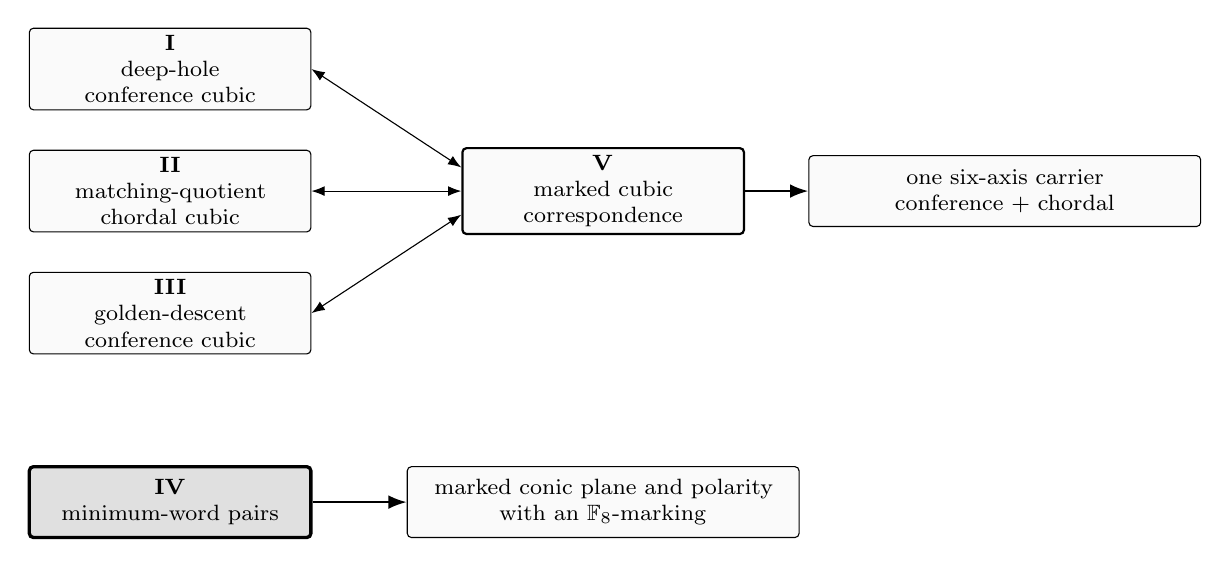
\begin{tikzpicture}[
  x=1cm,y=1cm,>=Latex,
  paper/.style={draw,rounded corners=1.5pt,fill=black!2,
    align=center,font=\footnotesize,minimum height=9mm,text width=34mm,
    inner sep=2.5pt},
  active/.style={paper,very thick,fill=black!12},
  hinge/.style={paper,thick},
  package/.style={paper,text width=48mm}
]
\node[paper]   (p1) at (0,1.9) {\textbf{I}\\deep-hole\\conference cubic};
\node[paper]   (p2) at (0,0.35) {\textbf{II}\\matching-quotient\\chordal cubic};
\node[paper]   (p3) at (0,-1.2) {\textbf{III}\\golden-descent\\conference cubic};
\node[hinge]   (p5) at (5.5,0.35) {\textbf{V}\\marked cubic\\correspondence};
\node[package] (gold) at (10.6,0.35) {one six-axis carrier\\conference \(+\) chordal};
\node[active]  (p4) at (0,-3.6) {\textbf{IV}\\minimum-word pairs};
\node[package] (plane) at (5.5,-3.6) {marked conic plane and polarity\\with an \(\F_8\)-marking};
\draw[<->] (p1.east) -- ([yshift=3mm]p5.west);
\draw[<->] (p2.east) -- (p5.west);
\draw[<->] (p3.east) -- ([yshift=-3mm]p5.west);
\draw[->,thick] (p5.east) -- (gold.west);
\draw[->,thick] (p4.east) -- (plane.west);
\end{tikzpicture}
\caption{Programme map.  The upper double arrows are Paper~V's marked
transports and returns between the chordal and conference shadows; the right
arrow is its common-carrier reconstruction.  The lower solid arrow is
Paper~IV's independent minimum-word reconstruction.  Only the residual
\(C_2\)- and Frobenius-orbit markings are compared across the two branches.}
\label{fig:programme-map}
\end{figure}

The five papers are logically independent; the map records reconstruction
correspondences and thematic relations, not proof dependencies.

Here the sparse shadow is literal: the \(364\) minimum words of the binary
conic code are the starting data.  Unary support data are constant, while
weighted pair concurrences recover the marked conic plane and its polarity,
so the exact reconstruction arity is two.

The theorem is logically independent of the other Clebsch papers; its place
in the programme is methodological.  A different sparse shadow---minimum-word
pairs rather than syndrome or cubic data---again determines a much richer
source structure.

\begin{thebibliography}{9}

\bibitem{BallLavrauw2019}
S.~Ball and M.~Lavrauw,
\newblock Arcs in finite projective spaces,
\newblock \emph{EMS Surveys in Mathematical Sciences} \textbf{6} (2019),
133--172.
\newblock arXiv:1908.10772.

\bibitem{DromsMellingerMeyer2006}
S.~V.~Droms, K.~E.~Mellinger, and C.~Meyer,
\newblock LDPC codes generated by conics in the classical projective plane,
\newblock \emph{Designs, Codes and Cryptography} \textbf{40} (2006),
343--356.
\newblock doi:10.1007/s10623-006-0022-6.

\bibitem{HollmannThesis1982}
H.~D.~L.~Hollmann,
\newblock \emph{Association schemes},
\newblock Master's thesis, Eindhoven University of Technology (1982).

\bibitem{HollmannXiang2006}
H.~D.~L.~Hollmann and Q.~Xiang,
\newblock Association schemes from the action of
\(\PGL(2,q)\) fixing a nonsingular conic in \(\PG(2,q)\),
\newblock \emph{Journal of Algebraic Combinatorics} \textbf{24} (2006),
157--193.
\newblock doi:10.1007/s10801-006-0005-8; arXiv:math/0503573.

\bibitem{MadisonWu2012}
A.~L.~Madison and J.~Wu,
\newblock On binary codes from conics in \(\PG(2,q)\),
\newblock \emph{European Journal of Combinatorics} \textbf{33} (2012),
33--48.
\newblock doi:10.1016/j.ejc.2011.08.001; arXiv:1104.0324.

\bibitem{MaLiuTian2024}
L.~Ma, S.~Liu, and Z.~Tian,
\newblock The binary codes generated from quadrics in projective spaces,
\newblock \emph{AIMS Mathematics} \textbf{9} (2024), 29333--29345.
\newblock doi:10.3934/math.20241421.

\bibitem{Tranchida2024}
P.~Tranchida,
\newblock Triples of involutions in \(\PGL(2,q)\) and their incidence
geometries,
\newblock \emph{Innovations in Incidence Geometry} \textbf{22} (2025),
no.~1--2, 25--46.
\newblock doi:10.2140/iig.2025.22.25; arXiv:2411.10299.

\end{thebibliography}

\enlargethispage{5\baselineskip}
\section*{AI assistance disclosure}

This project was developed with extensive assistance from OpenAI Codex and
Anthropic Claude. Under the author's direction, the systems assisted with
proof exploration, literature research, symbolic and finite computation,
code and formal-proof development, verification, and manuscript drafting and
revision. The author checked the resulting arguments, computations, code,
and cited sources, reviewed and edited all AI-assisted material, and assumes
responsibility for all content.

\end{document}
